\chapter{Environment Setup for Application Development}
\label{appendix:env_setup}

The environment setup procedures for the development of the IR web application are presented here. The procedures described below are based on Windows 10 host platform, with Intel Core i7-4700HQ processor, 8 GB RAM, and 1 TB HDD. For other operating systems or other system specifications, users may follow similar procedures to set up the environment but specific settings or installation may vary.

\section{Install Ubuntu Virtual Machine}
\subsection{Install VirtualBox} 
Visit VirtualBox's download page (\url{https://www.virtualbox.org/wiki/Downloads}).  Select the Windows installer and install the latest version in the same way as any normal Windows programs.

\subsection{Install Ubuntu} 
Get a Ubuntu disk image (.iso file) from Ubuntu's download page (\url{https://www.ubuntu.com/download/desktop}). Next, install Ubuntu inside Windows using VirtualBox. You may refer to instructions in \url{http://www.psychocats.net/ubuntu/virtualbox}.

Ubuntu 16.04 was used for the development. For your reference, Figure \ref{fig:vm_config} is the author's settings for the virtual machine. The settings should be applicable to most of the commercial laptops.

\begin{figure}[!htbp]
  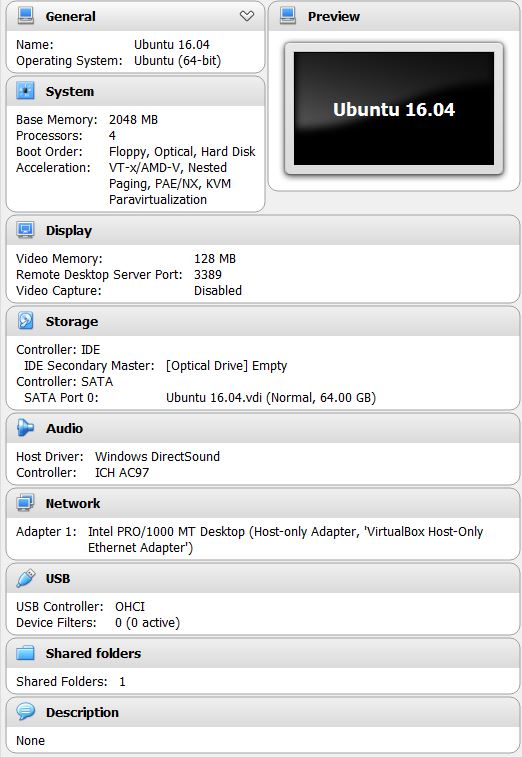
\includegraphics[width=.9\textwidth]{appendix/vm_config.jpg}
  \caption{Ubuntu Virtual Machine Configurations}
  \label{fig:vm_config}
\end{figure}

During development, we need to access the guest machine from the host. Thus, host-only networking is used to create a private Ethernet network consisting of the host and the guest only. You may identify the IP address of the virtual machine using the command:
\begin{verbatim}
hostname -I
\end{verbatim}

The IP address is likely to be 192.168.56.101. The Django application server would need to access the Ubuntu virtual machine via this IP address. However, there is no Internet access for host-only networking; thus, you may need to change to NAT networking when you perform Step \ref{step:host_servers}.

\section{Host Solr, Redis, and MySQL in Ubuntu}
\label{step:host_servers}
\subsection{Host Solr} 
Boot up the Ubuntu virtual machine. Solr comes in a pre-packaged form that requires very little other than JRE and Jetty. Install Solr by running the following commands from a terminal prompt:
\begin{verbatim}
curl -LO https://archive.apache.org/dist/lucene/solr/4.10.2/solr-4.10.2.tgz
tar xvzf solr-4.10.2.tgz
cd solr-4.10.2/example/
mv solr/collection1/ solr/dsp_collection/
\end{verbatim}

Make ensure that you are in the directory \path{./solr-4.10.2/example}. Start Solr server by executing the following command:
\begin{verbatim}
java -jar start.jar
\end{verbatim}

You may now access Solr admin page from the host machine using the URL \path{http://<guest_ip_address>:8983/solr}.

\subsection{Host Redis} 
Install Redis by running the following commands from a terminal prompt:
\begin{verbatim}
wget http://download.redis.io/redis-stable.tar.gz
tar xvzf redis-stable.tar.gz
cd redis-stable
make
\end{verbatim}

Make ensure that you are in the directory \path{./redis-stable}. Start Redis server by executing the following command:
\begin{verbatim}
redis-server redis.conf
\end{verbatim}

\subsection{Host MySQL}
Install MySQL by running the following commands from a terminal prompt:
\begin{verbatim}
sudo apt-get update
sudo apt-get install mysql-server
\end{verbatim}

During the installation process you will be prompted to enter a password for the MySQL root user. Once the installation is complete, the MySQL server should be started automatically. You can run the following command from a terminal prompt to check whether the MySQL server is running:
\begin{verbatim}
service mysql status
\end{verbatim}

If the server is not running correctly, you can type the following command to start it:
\begin{verbatim}
sudo service mysql restart
\end{verbatim}

\section{Create Python Virtual Environment in Windows}
\subsection{Install Python 3}
You may install the latest Python 3 version from Python's download page (\url{https://www.python.org/downloads/}). The Python package manager \texttt{pip} is included in Python 3.4 and above by default.

To access \texttt{pip} from any directory in the Command Prompt, make sure the \path{Scripts} subdirectory of Python is in the environment variable \texttt{PATH}. For example, if Python is installed in \path{C:\Program Files (x86)\Python\Python35-32\}, you should make sure \path{C:\Program Files (x86)\Python\Python35-32\Scripts} is in \texttt{PATH}.


\subsection{Install Virtual Environment Packages}
\texttt{virtualenv} is a tool to create isolated Python environments, each with their own libraries and site-packages. \texttt{virtualenvwrapper} is a set of commands which makes working with virtual environments much more pleasant. Both packages should be installed into the same global site-packages area inside Python's directory. You may need administrative privileges to do that. Install the two packages by running the following commands from Windows Command Prompt:
\begin{verbatim}
pip install virtualenv
pip install virtualenvwrapper-win  
\end{verbatim}

\texttt{virtualenvwrapper} places all virtual environments in one place. By default, they are placed in \path{%USERPROFILE%\Envs}. 

\subsection{Create Python Virtual Environment}
\label{step:create_vir_env}
Create a new virtual environment named \texttt{<name>} by running the following command in the Command Prompt:
\begin{verbatim}
mkvirtualenv <name>
\end{verbatim}

Activate the environment named \texttt{<name>} by running the following command:
\begin{verbatim}
workon <name>
\end{verbatim}

You may deactivate the working environment and switch back to the global environment by running the command:
\begin{verbatim}
deactivate
\end{verbatim}

\section{Clone Project from GitHub}
\subsection{Install Python IDE PyCharm}
PyCharm was the sole integrated development environment (IDE) for the entire project, including front-end and back-end development. It is strongly recommended because of its extensive developer-friendly features.

You may install PyCharm Professional from PyCharm's download page (\url{https://www.jetbrains.com/pycharm/download/}). If you are student, you may get free JetBrains license with your school email. More information is here: \url{https://www.jetbrains.com/student/}.

\subsection{Install Git}
Visit Git's download page (\url{https://git-scm.com/downloads}) and install the latest version of Git. Specify the location of the Git executable file on the \texttt{Git} page of the \texttt{Settings} dialog box in PyCharm. 

\subsection{Clone Project from GitHub}
Log in to your GitHub account in the \texttt{GitHub} page of the \texttt{Settings} dialog box in PyCharm. 

Next, we need to check out the project from GitHub. Choose \texttt{Checkout from Version Control | GitHub} in PyCharm. Set the Git Repository URL to be \url{https://github.com/HarveyLeo/myfyp.git}. You may set your local project location in the same dialog. Finally choose \texttt{Clone}. The source code is now cloned into your local directory.

\section{Install Required Python Packages}
Before you are ready to go, you need to install all the required python packages specified in \texttt{requirements.txt}. These are the packages necessary for the installation of technology stack mentioned in Section \ref{sec:tech_stack}.

Whenever you work on the project, make sure you are in the Python virtual environment created in Step \ref{step:create_vir_env}. You can go to the virtual environment by running the \texttt{workon} command, as mentioned earlier. After going to the environment, navigate to the project home directory \path{myfyp/} by using \texttt{cd} command in PyCharm Terminal. Next, install all required packages by running the following command:
\begin{verbatim}
pip install -r requirements.txt
\end{verbatim}

You may list all unused dependencies by running the command below and remove them using \texttt{pip uninstall}.
\begin{verbatim}
pip-autoremove --list
\end{verbatim}

\section{Configure Solr and MySQL}
\subsection{Update Ubuntu's IP Address in Settings}
Check Ubuntu's IP address and update the address in \texttt{settings.py}, which is located in the project directory \path{myfyp/myfyp/}. The IP address is set to 192.168.56.101 by default. You may replace all occurrences of this IP address in \texttt{settings.py} with Ubuntu virtual machine's actual IP address.

\subsection{Configure Solr Schema}
Generate Solr's \texttt{schema.xml} from Haystack by running the following command in PyCharm Terminal:
\begin{verbatim}
python manage.py build_solr_schema > schema.xml
\end{verbatim}

Make sure you are in the Python virtual environment named \texttt{<name>} before issuing the command above. Place the generated \texttt{schema.xml} inside the directory \path{solr-4.10.2/example/solr/dsp_collection/conf/}. Then restart Solr.

\subsection{Configure MySQL Database}
\subsubsection{Create Remote User Account and Database}
To grant remote access of MySQL database from any IP address, we need to create a user account in MySQL. Log in to the root account from a terminal prompt in the virtual machine using the command:
\begin{verbatim}
mysql -u root -p
\end{verbatim}

Enter the password that you created earlier for the MySQL root user. Once successfully logging in, run the following commands:
\begin{verbatim}
CREATE USER 'mysql-client'@'%' IDENTIFIED BY 'password';
GRANT ALL PRIVILEGES ON *.* TO 'mysql-client'@'%' WITH GRANT OPTION;
FLUSH PRIVILEGES;
\end{verbatim}

A new MySQL user account named \texttt{mysql-client} is hence created. The asterisks in the second command refers to databases and tables respectively that the account can access. This specific command allows the account to perform all tasks across all databases and tables. You may narrow the access privileges for this account later. To tell the server to reload the grant tables, a flush-privileges operation is performed by issuing the last command above.

Next, create a database named \texttt{dsp\char`_database} by running the command below in the \texttt{mysql>} prompt:
\begin{verbatim}
CREATE DATABASE dsp_database;
\end{verbatim}

\subsubsection{Change to UTF-8 Encoding}
To display the current character encoding set for the database \texttt{dsp\char`_database}, run the following command at the \texttt{mysql>} prompt:
\begin{verbatim}
SELECT default_character_set_name FROM information_schema.SCHEMATA 
WHERE schema_name = "dsp_database";
\end{verbatim}

If the character encoding is not UTF-8, convert to UTF-8 by running the following command at the \texttt{mysql>} prompt:
\begin{verbatim}
ALTER DATABASE dsp_database CHARACTER SET utf8 COLLATE utf8_unicode_ci;
\end{verbatim}

This does not convert existing tables. It only sets the default for newly created tables. However, at this stage there is no table in the database \texttt{dsp\char`_database}.

\subsubsection{Migrate Changes from Django Models}
You can now update the MySQL database named \texttt{dsp\char`_database} by running the following commands in PyCharm Terminal:
\begin{verbatim}
python manage.py makemigrations dsp_index
python manage.py migrate
\end{verbatim}

By running \texttt{makemigrations}, you are telling Django that you have made some changes to your models and that you would like the changes to be stored as a \textit{migration}. The \texttt{migrate} command takes all the migrations that have not been applied and applies those changes to the database.

\section{Start All Servers}
Before running the web application, you need to start Redis, Solr, and MySQL in Ubuntu; then, start Django application server and Celery worker server in PyCharm Terminal in Windows. When you are in the Python virtual environment named \texttt{<name>}, navigate to the project home directory \path{myfyp/} and start the application server by running the following command:
\begin{verbatim}
python manage.py runserver
\end{verbatim}

Open a new Terminal in PyCharm, go to the virtual environment, and start the Celery worker server by running the following \texttt{celery} command with \texttt{worker} argument:
\begin{verbatim}
celery -A myfyp worker -l info
\end{verbatim}

\texttt{myfyp} is the current Django project name and \texttt{-l} is to indicate the log level.

\section{Access Webpages through Browsers}
You are now ready to go! The homepage, django-admin page, dsplearn-admin page can be accessed respectively via the following URLs.
\begin{itemize}
\item Homepage: \path{http://127.0.0.1:8000/}
\item Django-admin page: \path{http://127.0.0.1:8000/django-admin/}
\item Dsplearn-admin page: \path{http://127.0.0.1:8000/admin/}
\end{itemize}

To log in to the django-admin page, you need to create a superuser - a user account that has control over everything on the site. Type the following command to create a new superuser in PyCharm Terminal:
\begin{verbatim}
python manage.py createsuperuser
\end{verbatim}

You would need to crawl document data from the Document Server and index into Solr before searching. Go to the dsplearn-admin page and crawl data now! It took approximately 1 hour to crawl 1000 sections. Once crawling is finished, you may build the search index in Solr following commands in Section \ref{subsec:index_build}.
